\chapter{Re-Designing Algebraic Attacks Beyond ElimLin} \label{ch:ElimLIn}
\section{ElimLin Overview}
Our initial algebraic cryptanalysis work on Simon was published in 2014. In 2015,   Raddum \cite{RaddumSimon} published another algebraic cryptanalysis on several different versions of Simon and have broken 16 out of 72 rounds on the largest existing version Simon128/256 using Elimlin with 20 P/C pairs of chosen plaintexts. Raddum's work also shows that ElimLin performs better when adding more P/C pairs.  
%\subsection{UNSAT Method}


%secrypt2016 
%TODO
 
However, it's hard to know what happens when we add even more P/C pairs. This is due to the limited computation power we have. A major difficulty with ElimLin is that so far it has been successful only for relatively simple lightweight ciphers.
For more complex ciphers
%%% full version maybe %%%
%%it is not clear if the attack makes big progress.
it seems to do things which are relatively trivial,
%However until now this has not been formalized.
%We do not know what trivial means.
%for example
e.g. equations generated do not penetrate deeply inside the cipher, or very slowly,
cf. %for example
slide 153 in Courtois' lecture notes \cite{SlidesAlgAllteach}.
% we observe that as the number
%of new linear equations grows,
%these equations penetrate more and more deeply inside the cipher for $2,3,5,\ldots$ rounds.

Our work aims to make some definite progress in the direction of distinguishing between trivial and non-trivial behavior for ElimLin. This is about how deeply an ElimLin attack penetrates. Previous experience shows that ElimLin only starts to work at a certain threshold. Before this threshold, again, nothing non-trivial can be observed even though slow penetration occurs. This is not really apparent in any of the current works or is lost in vast quantities of data generated in the computer simulations. 
%In this paper we are going to be the first to define what non-trivial means.

 In this chapter, we study ElimLin behaviours with randomly selected, increasing number of data samples. By collecting data from large simulations and deeply inspecting the different types of equations generated by ElimLin, we study
 
 \begin{enumerate}
 	\item The growth rate of equations generated by ElimLin
 	\item Where the higher growth rate comes from
 	\item If it is possible to predict when ElimLin will break a cipher
 \end{enumerate}
 
We define a new criterion which shows that it is possible to see that there exist two very different and easily distinguishable patterns in ElimLin. Either the attack follows one pattern, and does nothing non-trivial, or it follows another pattern and it is very clearly doing well. Then we look deeply inside the large number of linear equations found by ElimLin and try to classify different type of equations and identify where the higher growth rate come from.

\subsection{Phase transitions}

It is known that many NP-hard problems are subject to ``phase transition''; with certain parameters that problem is hard, and then it will rather abruptly transition from ``hard'' to ``easy to solve''. This is what we observe with ElimLin. % here. 
Let $K$ be the number of Plaintext/Ciphertext (P/C) pairs used in an ElimLin attack. We are going to discover that at a certain threshold the number of new linear and linearly independent equations
generated at various stages of the attack can follow one curve,
and then switch to another curve with a different asymptotic growth rate.



%\begin{conj}
{\bf Conjecture \ref{ElimLinQuadConj}}
\label{ElimLinQuadConj}
Consider a system of multivariate equations derived from a block cipher (see toy example in \ref{sec:AA} Figure \ref{fig:ch3ACmodeling}). %TODO
Consider a simple known plaintext attack with $K$ Plaintext/Ciphertext (P/C) pairs.
Consider a case such that the cipher is eventually broken by ElimLin, cf. \cite{FastAlg,FastAlg2,ToyRijSer,AlgteachElimLinLab,RaddumSimon}.
The number of new and linearly independent linear equations generated
by the ElimLin algorithm goes through several distinct stages St0-St3:

\begin{enumerate}
	\item[St0]
	Initially it grows linearly with $K$,
	and for certain individual stages of the attack is
	simply equal to 0 and does NOT grow,
	cf. our later $s_i$ notation in Section \ref{ElimLinNotation}.
	\item[St1]
	Then it switches to another curve where
	it grows faster than linearly in $K$.
	%cf Sec. \ref{SuperLinearGrowth}
	\item[St2]
	This is until it reaches a \textbf{saturation} stage where the
	cipher is completely broken by ElimLin.
	Here we sometimes have a very rapid phase transition (cf. Section \ref{BigPictureUpAndDown})
	where the number of equations $s_i$ generated at one stage becomes 0 again
	simply because an earlier stage of the attack reaches a certain threshold where combinatorial explosion
	in additional equations generated
	makes it complete the whole attack and does not requite the next stage to be executed.
\end{enumerate}

\noindent
%Again let $K$ be the number of P/C pairs in an ElimLin attack.
One (old) example from 2007 which shows that the number of equations grows faster than linear
as a function of the data complexity $K$ in ElimLin can be found in Courtios and Debraize's work in 2008 \cite{ToyRijSer}. 

In this chapter we would like to see if this conjecture is verified in real life and how exactly we can approximate different stages of the attack by precise closed formulas which allow us to predict the outcomes of the attack as exactly as possible. 

%A more detailed analysis on equations growth with respect to $K$ can be found in \ref{sec:elimlinJava}


%\newpage

%\section{\uppercase{Our Experimental Setup and Notation}}

\section{How to Predict the Success of ElimLin}

\subsection{Experimental Setup and Notation}
\label{ElimLinSetup}
\label{ElimLinNotation}

We recall the two main and only steps of ElimLin:

\begin{enumerate}
	\item[1] Find $s_i$ linear equations in the linear span, $i=0,1,2,3,\ldots$.
	\item[2a] If $s_i>0$ eliminate some $s_i$ variables,
	increment $i$ and try again Step 1.
	\item[2b] Algorithm terminates when $s_i=0$ for some $i$.
\end{enumerate}

In addition and by convention we are going to define a step $i=0$ which is different than
above, but the same as which is implemented in a common implementation of ElimLin \cite{CourtoisSoftware}.
We will assume that $s_0$ will be the number of linear equations which already appear in the equations,
without executing any linear algebra. This is a convention which allows researchers to distinguish
more easily between a ``misleading'' starting number of variables (which is sometimes artificially inflated due to
methods used for equation generation and formal coding)
and the ``real'' or intrinsic number of variables which is there prior to execution or ElimLin.

%\begin{defi}[ElimLin progress indicators]\\
\begin{mydef}\label{ElimLinProgressParams}
	[ElimLin progress indicators]\\
	Let $V_{start}$, or simply $V$ if there is no confusion,
	be the initial number of variables.
	We define by $s_i$ the number of
	linear/affine equations over GF(2)
	generated at each stage of the algorithm
	where by convention $s_0$ is the number of
	linear/affine equations over GF(2) already present.
	We define
	
	\begin{equation}
	V^i_{broken}=\sum_{j=0}^{i} s_j ~~~~~~~~V_{broken}=\sum_{i=0}^{\infty} s_i
	\end{equation}
	
	where by convention $s_i=0$ if algorithm has reached
	$V^i_{broken}=V$ at an earlier stage.
	We define also
	
	\begin{equation} \label{EQ:unborken}
	V^i_{broken}=V-\sum_{j=0}^{i} s_j
	\end{equation}
	
	and accordingly let
	$
	V_{unbroken}=V-\sum_{i=0}^{\infty} s_i.
	$
	Overall we will say that the algorithm terminates if
	$V_{broken}=V$ and $V_{unbroken}=0$ and we deliberately ignore the fact that
	some variables could be subject to a brute-force step,
	cf. FXL method introudced by Courtois and Patarin \cite{XL2}.
	Overall our goal is to achieve for a certain $i$ that
	\begin{equation}
	\frac{V^i_{broken}}{V_{start}}=1
	~~~~~~~~~~~\mbox{or}~~~~~~~~~~~~
	\frac{V^i_{unbroken}}{V_{start}}=0
	\end{equation}
	
\end{mydef}
%\end{defi}

To give an example of how the experiments are done\footnote{The same software setup has also been used at UCL to run a hands-on student lab session on algebraic cryptanalysis of block ciphers \cite{AlgteachElimLinLab}, which is part of GA18 course on cryptanalysis taught at UCL.}: our Simon implementation is available on GitHub  \cite{AlgteachElimLinLab,CourtoisSoftware}; The ElimLin is executed using one of our implementations of
ElimLin \cite{AlgteachElimLinLab,CourtoisSoftware} which has the nice ability to display on screen the number of linear equations generated at each stage/iteration of the algorithm. Finally we have developed a deep inspection tool in JAVA available online \cite{CourtoisSoftware} which looks deeply inside the equations generated by ElimLin, group the equations based on different selection criteria then provide statistics and predictions for the growth rate of each group. For detailed instructions about how to get these values and full experiment results, see appendix \ref{appendixlabel1}

\section{The Big Picture}
\label{BigPictureUpAndDown}

As already explained in
Conjecture \ref{ElimLinQuadConj}, we expect that there are at least 3 distinct stages in the ElimLin algorithm.
We start with the big picture, by looking at how the value of $V_{unbroken}$ evolves with growing $K$. Here we use a known plaintext setting with no guessed key bits to break 8 round Simon64/128. As we know, adding new P/C pairs to the ElimLin should create a linear growth in the total number of variables. In our experiment setup and Simon encodings, each P/C pair adds 192 variables to the starting equation system. Thus if we have two ElimLin runs, assume ElimLin solved $m_1$ and $m_2$ variables with $k_1$ and $k_2$ P/C pairs, the unsolved variables should equal to $192 k_1 - m_1 $ and $192 k_2 - m_2$.  We study the number of unsolved variables left at the end of ElimLin run. By looking at the gradient of the curve to study the growth rate of solved variables as a function of $K$ P/C pairs. Our results are shown in Figure \ref{ElimLinUnrokenCurveUpDownSimon8} with a fitting curve using polynomial regression.

\begin{figure}[h!]
	\vspace{-0.2cm}
	\centering
	\includegraphics*[width=140mm,height=13cm]{./pics/Figure6-1.png}
	\caption[Number of variables when ElimLin terminates  $V_{unbroken}$
		for 8 rounds of Simon 64/128 obtained with our experiments.]{Number of variables when ElimLin terminates  $V_{unbroken}$
			for 8 rounds of Simon 64/128 obtained with our experiments.
		When $K \leq 16$ the unbroken variables increase. Variables solved by ElimLin are less or equal than variables increased due to added new P/C pairs. We consider this is St0 in
		Conjecture \ref{ElimLinQuadConj}. When $ 16 < K \leq 50 $ the unsolved variables start to slowly decrease, we consider this is St1. When $ K > 50 $ unbroken variables decrease much faster than linear and we consider this stage as St2.}
	\label{ElimLinUnrokenCurveUpDownSimon8}
	\vspace{-0.1cm}
\end{figure}

In Figure \ref{ElimLinUnrokenCurveUpDownSimon8}, we can see a distinction between St0 and St1. In St0 the number of unbroken variables grows linearly with $K$. When the curve switches to St2, the number of unbroken variables grows much more slowly. This curve shows that the number of new generated equations is growing much faster than linear in St1 and causing a lot of variables eliminated by ElimLin. Clearly, St1-2 is the most fundamental stages of ElimLin. It contains the phase transition from ``hard" to ``easy".



\subsection{On Growth Rate in ElimLin}
\label{SuperLinearGrowth}
In section \ref{BigPictureUpAndDown} we looked at the overall unbroken variables as a function on $K$ P/C pairs. We know the total varible growth linearly with $K$. So based on equation \ref{EQ:unborken} we know the solved variables increase faster than linear in St2. Here we look at the growth rate on the number of newly generated equations as a function of $K$.  On Figure \ref{fig:ElimLinQuadConjExampleSimon8r123} we show that early stages $s_{0,1,2,3}$ (see definitions in Section \ref{ElimLinNotation}) of ElimLin algorithm on 8 rounds of Simon block cipher grows linearly. This means at the early stage, ElimLin algorithm only finds trivial equations and the results are very easy to predict. 

Moreover a linear progress curve would not be sufficient to break the cipher, 
because the number of variables also increases linearly. 
In addition, initially the attack starts with a handicap: below a certain threshold no equation exist at all, or many types of equations (equations with similar size and
characteristics, topic which we will study later) seen in larger simulations do not yet exist at all (0 equation found).



\begin{figure}[!h] 
	\vspace{-0.2cm}
	\centering
	\includegraphics*[width=160mm, height=14cm]{./pics/s1s2s3asK.png}
	\caption[Number of linearly independent equations generated at step 1,2,3
	of the ElimLin algorithm]{Number of linearly independent equations generated at step 1,2,3
		of the ElimLin algorithm
		for 8 rounds of Simon 64/128. The results show in step 1,2,3 of ElimLin, number of equations increase linearly and does not create the faster than linear growth we oberseved in Figure \ref{ElimLinUnrokenCurveUpDownSimon8}.}
	\label{fig:ElimLinQuadConjExampleSimon8r123}
	\vspace{-0.1cm}
\end{figure}

In Figure \ref{fig:ElimLinQuadConjExampleSimon8r4}, we show the number of linear equations generated at step 4 of the ElimLin algorithm for 8 rounds of Simon block cipher. We have then produced a polynomial interpolation for this data series. It grows faster than linear which is the first stage of the attack with a positive and non-trivial outcome. 

\begin{figure}[!h]
	\vspace{-0.2cm}
	\centering
	\includegraphics*[width=150mm,height=12cm]{./pics/s4asK.png}
		\caption[Number of linearly independent equations generated at step 4]{Number of linearly independent equations generated at step 4
			of the ElimLin algorithm
			for 8 rounds of Simon 64/128. Step 4 equations appear at K=16, and shows faster than linear increase when $K > 50$, this algains with the stages appeared in Figure  \ref{ElimLinUnrokenCurveUpDownSimon8} when curve switch from St0-1 and St1-2. }
	\label{fig:ElimLinQuadConjExampleSimon8r4}
	\vspace{-0.1cm}
\end{figure}

Note that we start to have $s_4 > 0$ when $K >16$. This also aligns with Figure \ref{ElimLinUnrokenCurveUpDownSimon8} when we see a switch from St0 to St1. 
This is where ElimLin starts to create a growing number of equations which we want to 
grow faster than linear. 
 
\subsection{Deep Inspection}
We start to wonder \textbf{which} set or type of equations in $s_4$ grows faster than linear. 
Up till now we still don't know what kind of equations are found when ElimLin starts to work, and we conjecture that precisely those equations with a fast growth rate are particularly significant and could be a sort of - up to - primary reason why we can break the cipher for some parameters, or in combination with other equations. 
So we have designed and programmed an open-source inspection tool called ``DeepElimlin" \cite{CourtoisSoftware} to look inside the large number of equations generated by ElimLin and to classify these equations into many detailed types or classes and to visualize and analyse these types in detail. We conjecture that the hardest equations that can be found by are equations that use many different P/C paris and involes variables in the middle of the encryption. Thus, we decided to group the equations in subcategories by 

\begin{enumerate}
	\item The number of distinct instances (P/C pairs) used: J, where $J \leq K$.
	\item The ElimLin execution stage: $r$.
	\item The penetration rounds: 
	maximal and minimal round involved in any of the variables: $R_{max}$ and $R_{min}$. 
\end{enumerate} 

We postulated that in most cases the maximal round is the round which is the most deeply embedded or close to the middle round. It is the hardest round to penetrate for any attack, as a matter of fact. Importantly, sometimes we will find equations use variables from both sides (penetrating from both plaintext and ciphertext). 
In this case we just use the smallest round as minimal and largest round as maximal. 
It is also important to see that the cipher cannot be broken as long as equations which combine penetration from both sides are not yet generated. This is because equations on the plaintext side could be computed without the knowledge of the ciphertext and vice versa. Then we don't expect to be able to mix these equations very well in the solving process, and identify smaller equations having maybe a unique solution at the end of the solving process, and we don't expect to increase the degree so much that the equations would really interact. 

We create sub-categories based on each distinct combination of these values. An example of one equation found in $s_4$ is given in Figure \ref{fig:DeepLin1}, where key variables are compressed as $k\_\{Keybit+Keybit+...\}$; the intermediate variables (input at each round) are named based on $ZR\left[\text{instance}\right]\_\left[ \text{round}\right]\_\left[bit\right] $. In this example we have $J=3$, $s = 4$, $R_{max} = 4$ and $R_{min}=5$. This equation belongs to subcategory ``s4J3R5-4". 

\begin{figure}[h!]
	\vspace{-0.2cm}
	\centering
	\includegraphics*[width=160mm]{./pics/ElimLinDeep.png}
	\caption[Example of a non-trivial equation found by ElimLin]{Example of a non-trivial equation found by ElimLin. The example equation contains variables from 3 different P/C pairs (ZR1,ZR2 and ZR3), variables appears in mutiple middle rounds (4th and 5th round of encryption). Such equations are considered as non trival equations and increasing faster than linear during ElimLin calculations}
	\label{fig:DeepLin1}
	\vspace{-0.1cm}
\end{figure}

Then we found a few sub-categories in $s_4$ in which the number of equations grows much faster than linear, see Table \ref{tab:Jason3col}:

\begin{table}[h!]
	\caption[Example of equations growing faster than linear as a function of $K$]{Example of equations growing faster than linear as a function of $K$. This table shows a selected group of equations that grow faster than linear as a function of $K$. These equations start to appear after $K \geq 16$ in step 4 (cf. Figure \ref{fig:ElimLinQuadConjExampleSimon8r4}). Equation group defintaion is explain above, subcategroy s4J4R3-6 means equations contains variables using 4 P/C pairs, variables in 3 to 6 round of Simon encryption.  }\label{tab:Jason3col} \centering
	\label{Tab:SplitS4in3main}
\begin{tabular}{|c|c|c|c|}
	\hline
	\# of P/C pairs& 16 & 32 & 64 \\ \hline
	s4J2R3-6 & 2  & 4  & 31 \\ \hline
	s4J3R3-6 & 2  & 6  & 54 \\ \hline
	s4J4R3-6 & 1  & 6  & 17 \\ \hline
\end{tabular}
\end{table}

We discover that faster-than-linear growth happens when the variables meet in the middle. 
%However we can't draw any conclusion yet as we did not do enough simulations. 
We have also discovered that the curve of Figure \ref{fig:ElimLinQuadConjExampleSimon8r4} splits into different  categories in a relatively stable way, so that the curve can be viewed as essentially a sum of 3 curves 
of Table \ref{Tab:SplitS4in3main} and other smaller terms. However it appears that this splitting process depends on ElimLin's order of elimination. 
More precisely linear combinations of certain types of equations will sometimes (rare cases) not be reported in our statistics because they are linearly dependent w.r.t other categories we study. 
A fully objective classification would require costly computations of the shortest possible basis for our linear space. 
This is actually not a problem we have observed here, but we have seen such ambiguities in experiments with our later scaling down heuristic, cf. next section. Current theory only guarantees that the full result of ElimLin is independent on the order of variables \cite{ElimLinRevisit}. 

\section{Known Plaintext vs Chosen Plaintext}
\paragraph{Scaling Down Method} \mbox{} \\
One idea behind the scaling method is we can find equations generated for a smaller $K$ inside a larger simulation, if the order of elimination allows it (sometimes they could be linearly combined with other equations). A second idea is that, therefore, just one large ElimLin simulation reveals a lot of information about smaller simulations and about the scalability of the results as $K$ grows. We developed a scaling down software (inside DeepElimLin) which will estimate the number of equations which could be found in a smaller $K'$. However, such predictions are not always very accurate. 

Given a set of equations $E$ generated by ElimLin with $K$ instances, we estimate the number of equations for $K' < K$ as follows:

For each equation $e \in E$, count the equation if the largest index of instance $k < K'$ 
 
One example which we found scaling down method works well is the following: in a chosen plaintext model for 32 round of Simon64/128, where we chose $K=64$ plaintexts in a counter mode, we obtain structured plaintext data and random ciphertext data. We call a cube any such set of plaintexts. 
Some of these equations will be actually adding the ciphertexts for all the points in the cube, which will be exactly as in the so-called cube attack well-known in the literature \cite{dinur2009cube}. However, many others just consider some of the outputs, and therefore we also discover lots of equations which have plaintexts which form a cube, but which are a lot more complex and may contain arbitrary sums of arbitrary single output bits.  
Below we present some results extracted from a very large simulation series.
 
\begin{table}[h!]
	\caption[Scaling down method results for 32 Rounds Simon]{Example of how scaling down method works well in a Chosen Plaintext Attack (CPA) for 32 round Simon64/128. As running ElimLin for large number of rounds takes a lot of computational resource, we argue that one can run one experiment (say K=64) and scale down to predict the performance of equations generated by a smaller number of P/C pairs (say K=32). Instead of running both experiments. Scaling down method can save us time to run experiment and the results are relatively relaiable at least for the earlier rounds. This table also shows that when selecting structured P/C pairs, ElimLin can penetrates more rounds and found more linear relations in deeper rounds compare to Known Plaintext Attack (KPA) in the ciphertext side. The results also align with our work in Chapter \ref{ch:SIMON}. } \label{tab:scallingdownworks} \centering
	\begin{tabular}{|c|c|c|c|}
		\hline
		& Real 32 & Predicted 32 & Real 64 \\ \hline
		R2  & 224     & 225.17     & 448     \\ \hline
		R3  & 448     & 419.67     & 848     \\ \hline
		R4  & 372     & 336.17     & 716     \\ \hline
		R5  & 104     & 68         & 279     \\ \hline
		R6  & 123     & 56.17      & 327     \\ \hline
		R7  & 118     & 61.83      & 314     \\ \hline
		R8  & 63      & 41         & 176     \\ \hline
		R28 & 1       & 0.83       & 4       \\ \hline
		R31 & 1024    & 1029.33    & 2048    \\ \hline
	\end{tabular}
\end{table}

%Explain R2 R28 etc
R2 is a collection of results which has the deepest round of 2. R28 works backwards. 
The predicted results are averaged based on all possible subsets with the size of $K'$ out of $K$. 

We observe that Chosen Plaintext side penetrates more rounds than the Known Plaintext side, and the equations are shorter and less complex. Predictions are less accurate in the deeper rounds.
%Known plaintext side has a linear growth rate close to 32$K$...
 
 
\section{Equations In ElimLin vs. Direct Approximation} \label{Sec:ElimLinVsApprox}
\vskip-5pt

Given $K$ random plaintexts,
how many linear equations are true for every key 
which combine variables from $K$ copies of 32 variables
inside round $Nr$ of encryption?
In addition we know the $K$ plaintexts and will study the equations which exist for some fixed $K$ plaintexts, which means that we will in general find more equations than those true for every plaintext. However, such equations are allowed in ElimLin attack where the plaintext is known.
We should also note that many such equations do not depend on the plaintext (some do),
and typically the total number of such equations does not depend a lot on
the choice of $K$ random plaintexts,
though it will be substantially bigger
in a Chosen Plaintext Attack (CPA) which penetrates deeper inside the cipher (see Chapter \ref{ch:SIMON}). 
%Link to Chapter 5 simon 
%cf. \cite{desalg,FastAlg,FastAlg2}.
%which other?  ,ToyRijSer,AlgteachElimLinLab}

These equations can be computed by standard linear algebra method:
we need to compute a kernel of a certain Macaulay matrix
[classical method in algebraic cryptanalysis].
We write a matrix
in which lines are examples of internal data for different keys
and columns represent various monomials,
which are all linear in this case.
The number of keys should be slightly higher than the number of columns,
e.g. 100 more.
The computation of the kernel of this matrix gives
a basis for the equations which are true for every key and related to our
monomials. This is a heuristic method which works with a large probability close to 1. 
For example, if we have $P_i/C_i$ being the plaintext/ciphertext variables,
and $R_1,\ldots R_{100}$ are the internal variables,
we might discover that for every key and for a fixed plaintext $P$
we have
$R_2\oplus R_7=1$. This is, of course, just an example.

\subsection{Polynomial Approximation in Practice}

We have programmed this method of recovery of the equations from the data.
%vs. those eventually discovered in ElimLin (maybe less).
The command line is:


\begin{verbatim}
ax64 9051777 32 128 Nr K 0 /fix80 /seed1
\end{verbatim}
%predict_905177_4R_fix80_KP.xlsx
%predict_905177_7R_fix80_KP.xlsx

This recovers the equations in a totally general Known Plaintext (KP) attack with random
plaintexts.
For example we obtain:
\begin{verbatim}
ax64 9051777 32 128 6 2 0  /fix80 /seed1-100
0.05 found on average
ax64 9051777 32 128 6 4 0  /fix80 /seed1-100
0.45 found on average
ax64 9051777 32 128 6 8 0  /fix80 /seed1-100
3.4 found on average
\end{verbatim}

We have analyzed the results obtained for $6$ and $7$ rounds
% we give series of points
and we obtained:

\vskip-4pt
\vskip-4pt
$$
F(6)\approx 0.0002 K^2 + 32 K - 724
$$
\vskip-4pt
%see predict_905177_6R_fix80_KP.xlsx

\vskip-4pt
\vskip-4pt
$$
F(7)\approx 0.00003 K^2 + 32 K - 12848
$$
\vskip-4pt
%see last few vals in predict_905177_7R_fix80_KP.xlsx !!!
%predict_905177_4R_fix0_KP.xlsx

More generally we conjecture that the quadratic part would disappear for larger $K$, and it is possible to show that:

\begin{lemma}[Theoretical Upper Bound on ElimLin Attack]
	\label{Lem:UppBoundKP}
	The number linear equations which ElimLin can find in KPA scenario
	is at most:
	$$
	F \leq 32 K - (T-\kappa)
	$$
	where $\kappa$ is the key size,
	$T$ is the cardinal of the union of the sets of monomials in $k_i$
	which appear in the union of ANF expressions
	(Algebraic Normal Forms are simply polynomials over $\mathbb{F}_2$)
	of all outputs of the cipher as a function
	of the key variables $k_i$ and plaintext variables. %, for a fixed set
	of $K$ plaintexts.
	
	Moreover (in practice) this number $T-\kappa$
	does not change when we select another set of $K$
	random plaintexts and for larger $K$ we have:
	
	$$
	F_{K\to\infty } \to 32 K - (T-\kappa)
	$$
	
	and starting from a certain threshold $K$ we typically have $F = 32 K - (T-\kappa)$ exactly (experimental).
	
\end{lemma}

\vskip-5pt
\noindent\emph{Proof (Sketch):}
For one plaintext $P_i$ each output is a Boolean function
which involves a certain number $T(P_i)$ of monomials in the $k_j$.
Moreover if we concatenate sets of monomials for several plaintexts
we expect to quickly reach an upper limit $T(P_i)\leq T$ where $T$
is the total number of monomials in the $k_j$ in the 32 polynomials
which are functions of both $P_i$ and the $k_j$.
For every $P_i$ the polynomials contain a subset of these $T$ monomials. 

For a fixed plaintext we form a Macaulay matrix
in which lines are different keys and different encryptions,
and columns are $32 K$ variables corresponding to $ZL_i$ after round $Nr$
(left hand side created in $Nr$ round of Simon encryption $i$ out of $K$),
plus $\kappa$ key variables.
Then it will have at most $T$ linearly independent columns,
as all columns could be written as linear combinations of other columns
which could be added for all possible monomials in key variables, and
the $\kappa$ linear monomials in key variables are those which we already had
in equations found by our software.

It is hard to prove $F=32 K - (T-\kappa)$ exactly for larger values, but this is what we observe in practice in algebraic cryptanalysis, for example \cite{XL2} and here. 

\paragraph{Experimental Results} \mbox{} \\
Here we present a more elaborate example than in our Proposition \ref{Lem:UppBoundKP}. 
Our experience show that results of experiments can be predicted with near 100$\%$ accuracy and 
there is typically more than one interval where the number of linear dependencies follow a linear curve 
with different values of $T$ and for a subset of 32 bits. Our interpretation is that 
the same sort of result holds for a subset of output bits however for some subsets the value $T$ is smaller because they depend on less key bits.
Our experiment results for 8R Simon64/128 KP are given in Figure \ref{fig:FullResBig}. It is clear to see that there are three different stages before it reaches $F = 32 K - (T-\kappa)$. For a smaller $K$ we observe $F = 6K - T'$ and then increase to $F = 27K - T''$, where $T'<T''<T$.

\begin{figure}[h!]
	\centering
	\begin{minipage}[b][22cm][b]{12cm}
		\begin{turn}{90}
			\includegraphics*[width=220mm, height = 120mm]{./pics/ch6BigScreen.png}
			\end{turn}
			\end{minipage}
			\begin{turn}{90}
				\begin{minipage}[c][1cm][c]{22cm}
					\caption{Experiment results for 8R Simon64/128 for theoretical upper bound on ElimLin attack }
					\label{fig:FullResBig}
					\end{minipage} 
					\end{turn}
					\end{figure}

Here we also privide an example of ElimLin not finding as many equations as in theoretical upper bound in Table \ref{tab:ElimLinVsUpperBound}.
\begin{table}[h!]
	\centering
	\caption[ElimLin vs Upper bound]{ElimLin vs Upper bound. We show the number of linear equations actual found by ElimLin and the theoretical upperbound for $K = 1,2,4 ... 64$. ElimLin can only found a subset of equations compare to the theoretical upperbound}
	\label{tab:ElimLinVsUpperBound}
	\begin{tabular}{|c|c|c|c|c|c|c|c|}
		\hline
		\# of P/C pairs& 1 &	2	& 4 &	8	& 16	& 32	&  64 \\ \hline
		ElimLin R4    & 11 & 28.82 & 46.63 & 86.39 & 167.77 & 336.17 & 716  \\ \hline
		Max Theor. R4 & 23 & 95    & 119   & 247   & 503    & 1015   & 2039 \\ \hline
	\end{tabular}
\end{table}

\paragraph{Application --- Prediction of Attack Complexity}
In our research we have NOT yet achieved our goal to be able to reliably predict the complexity of ElimLin attacks which we cannot yet run; but our SECRYPT paper results covered in this and previous sections suggest that this is feasible and here is one possible method to achieve it. 

\begin{conj}[Application of Proposition \ref{Lem:UppBoundKP}] \label{Con:ElimLin}
We can use the estimation of type $32K-C$ for the number of linearly independent equations 
which propagate from the plaintext side, another $32K-C$ which will be obtained from the ciphertext side, 
and estimate that the whole cipher is broken by a meet-in-the middle attack when $2(32K-C)\approx 32K$. 
Then we can estimate how many additional equations need to be added to ElimLin to complete, 
and we should be able to conclude that ElimLin+ attack (cf. next section) 
will break $2Nr$ of rounds as soon as this lower threshold is met. 

This method requires more development in terms of comparing the estimations to actual large ElimLin runs 
but we are the first to ever propose a plausible method to extrapolate the complexity of an improved 
form of ElimLin attack. 
\end{conj}

\section{Conclusion and Future Work}
ElimLin is a simple algorithm and works well for small number of rounds. Like other solving tools for Algebraic Cryptanalysis, it does not scale for larger number of rounds due to solving complexity. For a long time in Algebraic Cryptanalysis research, ElimLin was just used as a black box solving tool. In this chapter, we looked inside ElimLin algorithm and studied the equations generated by ElimLin at different solving stages. Contributions in this chapter are:
\begin{itemize}
	\item We introduced the phase transistions in ElimLin algorithm and expeimentally showed such phase transistions exist in many ciphers. 
	\item By looking at the number of linear independent equations found by ElimLin as a function of P/C pairs, We have identified the source and the nature of cryptanalytic success of ElimLin. It comes from several phenomena: equations emerge by thresholds, they meet in the middle, they exhibit super-linear growth in some (crucial) cases.
	\item We have also discovered how to efficiently generate a lot more equations which ElimLin does not typically find and provided a possible future application of ElimLin in Conjecture \ref{Con:ElimLin} 
\end{itemize}
We have all the ingredients. However, designing a really optimal algebraic attack on a block cipher is not an easy task due to the large complexity of the equations we have discovered. We feel that each class of equations could be computed faster by a dedicated method, and we have already computed many substantially faster by our Polynomial Approximation method above. Future research is needed on how ElimLin needs to be enhanced in practice and what kind trade-offs can be observed between the cost of computing various classes of equations we have already seen and others we have not yet fully integrated in ElimLin algorthim. In Section \ref{ElimLin+} we will review the works we have done in Part \ref{Part2} and discuss the plan of our future work on Algebraic Cryptanalysis.

\subsection{Algebraic Attacks Beyond ElimLin} \label{ElimLin+}
Many researchers consider algebraic cryptanalysis as an independent cryptanalysis research area called deterministic cryptanalysis, while differential and linear cryptanalysis methods are called probabilistic methods in cryptography \cite{pasalic2009probabilistic}. However, we argue that there are a lot of connections between algebraic cryptanalysis, linear and differential cryptanalysis. In Figure \ref{fig:ch3general}, we describe our view of the connections between these cryptanalytic techniques.

\begin{figure}[h!]
	\centering
	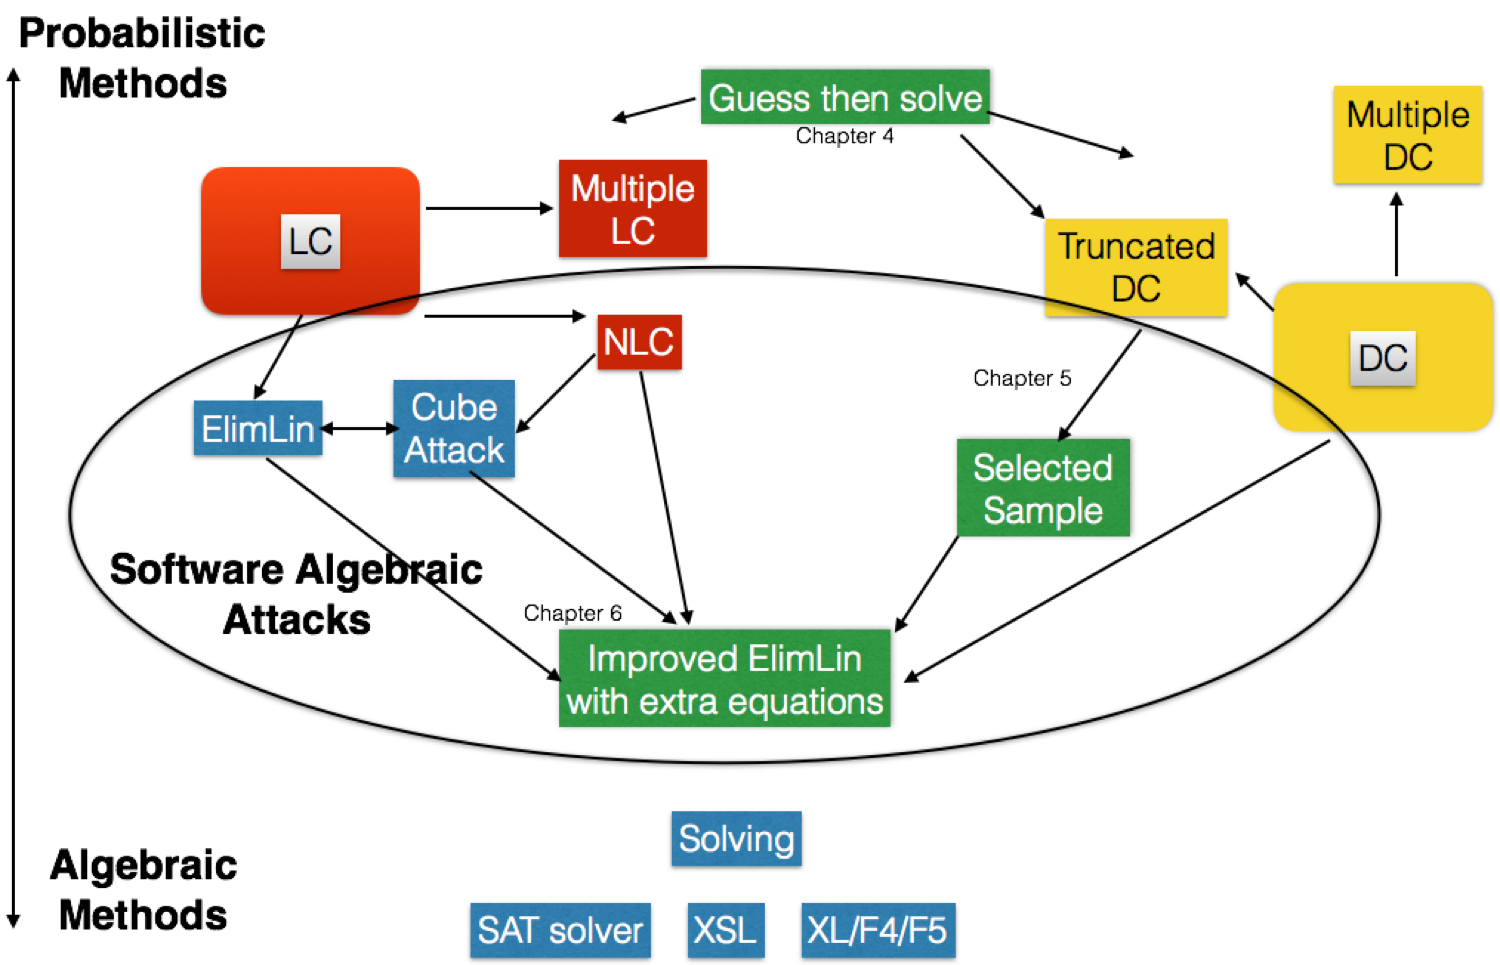
\includegraphics[width=130mm]{./pics/ch3general.png}	
	\caption[Classification of cryptanalysis methods and their connections]{Classification of cryptanalysis methods and their connections. Most of the existing literature considered algebraic cryptanalysis as an independent research area compare to probablisitic cryptanalysis methods such as differencial cryptanalysis (DC) and linear cryptanalysis (LC). We believe Algebraic Attacks has many connections. probablisitic method are often used together with Algebraic methods and in some attacks presented in this thesis they improved Algebraic Attacks performance by introduction new equations to the mathematic model and reduced solving complexity at the solving stage of Algebraic Attacks. Boxes colored in red are normally considered as LC. Yellow boxes are normally considered as DC methods. Green boxes are the parts included in this thesis and blue boxes are considered as specific solving methods}
	\label{fig:ch3general}
\end{figure}	

A link between ElimLin and linear cryptanalysis in Figure \ref{fig:ch3general} reflects the fact that both of these methods are looking for linear relations inside the cipher. However, a major difference between these two approaches is ElimLin looks for equations that work only for a particular set of P/C pairs\footnote{although some equations might exist for any P/C pairs}. Cube attack which was introduced by Dinur and Shamir in 2009 \cite{dinur2009cube} chooses a subset of 'public' input bits such that the sum of an output bit value is a linear combination of the key after a certain summation over a cube composed of plaintexts where a subset of bits varies. Cube attack can sometimes be linear and sometimes non-linear which can be seen as related to both ElimLin and Non-Linear Cryptanalysis (NLC) sometimes called Generalized Linear Cryptanalysis (GLC). Researchers have studied how well-selected samples from cube attack can be used to improve the performance of ElimLin\cite{suvsil2016selection} . One key focus is how different cryptanalysis techniques can be used to improve software algebraic attacks by adding more equations which makes that these attacks themselves will find yet more equations (amplification effect). 

Guess-then-solve method is a general cryptanalysis method which can be used in many attack scenarios. In Chapter \ref{ch:GOST} we explored this type of attacks on Russian GOST cipher and show this method can be used to improve algebraic cryptanalysis with SAT solvers. In Chapter \ref{ch:SIMON} we discussed how well-selected samples following a truncated differential property can reduce the solving complexity of ElimLin and SAT solvers. Both methods can be considered as adding additional linear equations into algbraic solving stage.

In Section \ref{Sec:ElimLinVsApprox} we discussed the theretical upper bound of equations that can be found by ElimLin. We conjectured that one can precompute additional linear equations that cannot be found by ElimLin, and provid those equations at the begining of solving step. We call \textbf{ElimLin+} any attack which combines ElimLin with additional equations generated by polynomial approximation as in this chapter. Our future work directions will consider to develop an attack using ElimLin+ on a concrete cipher and show it can break larger number of rounds than normal ElimLin method.